%% fig_frontier.tex   (generated by make_frontier.py; do not edit by hand)
%% The rule set with the routes of the literature: four minimal sufficient sets.
\documentclass[tikz,border=8pt]{standalone}
\usepackage{amsmath,amssymb}
\usetikzlibrary{arrows.meta,calc,decorations.pathreplacing}
%% palette.tex -- shared colour definitions for the figures
\definecolor{PInk}{RGB}{26,32,44}
\definecolor{PBlue}{RGB}{37,82,139}
\definecolor{PTeal}{RGB}{23,127,125}
\definecolor{POchre}{RGB}{193,138,44}
\definecolor{PClay}{RGB}{178,74,58}
\definecolor{PSlate}{RGB}{108,122,137}
\definecolor{PViolet}{RGB}{110,86,150}
\definecolor{WBlue}{RGB}{223,234,246}
\definecolor{WTeal}{RGB}{220,238,236}
\definecolor{WOchre}{RGB}{250,240,218}
\definecolor{WClay}{RGB}{247,229,224}
\definecolor{WSlate}{RGB}{238,241,244}
\definecolor{PMag}{RGB}{158,58,110}
\definecolor{PGrass}{RGB}{62,124,66}
\definecolor{PAmber}{RGB}{214,112,38}
\definecolor{PIndigo}{RGB}{58,64,140}
\definecolor{PRule}{RGB}{176,186,197}

%% shared macros so the standalone figures match the paper
\providecommand{\QQ}{\mathbb{Q}}
\providecommand{\ZZ}{\mathbb{Z}}
\providecommand{\RR}{\mathbb{R}}
\providecommand{\CC}{\mathbb{C}}
\providecommand{\PP}{\mathbb{P}}
\providecommand{\Kx}{K^{\times}}
\providecommand{\HW}{W}
\providecommand{\Nm}{\mathrm{N}}
\providecommand{\Hdg}{\mathrm{Hdg}}
\providecommand{\NS}{\mathrm{NS}}
\providecommand{\cA}{\mathcal{A}}
\providecommand{\cD}{\mathcal{D}}
\providecommand{\cF}{\mathcal{F}}
\providecommand{\cP}{\mathcal{P}}
\providecommand{\cO}{\mathcal{O}}
\providecommand{\cQ}{\mathcal{Q}}
\providecommand{\bbar}[1]{\overline{#1}}
\providecommand{\ch}{\operatorname{ch}}
\providecommand{\End}{\mathrm{End}}

\newcommand{\hcimp}{\,\textcolor{PIndigo}{\tiny$\Leftarrow\mathbf{HC}$}}
\begin{document}
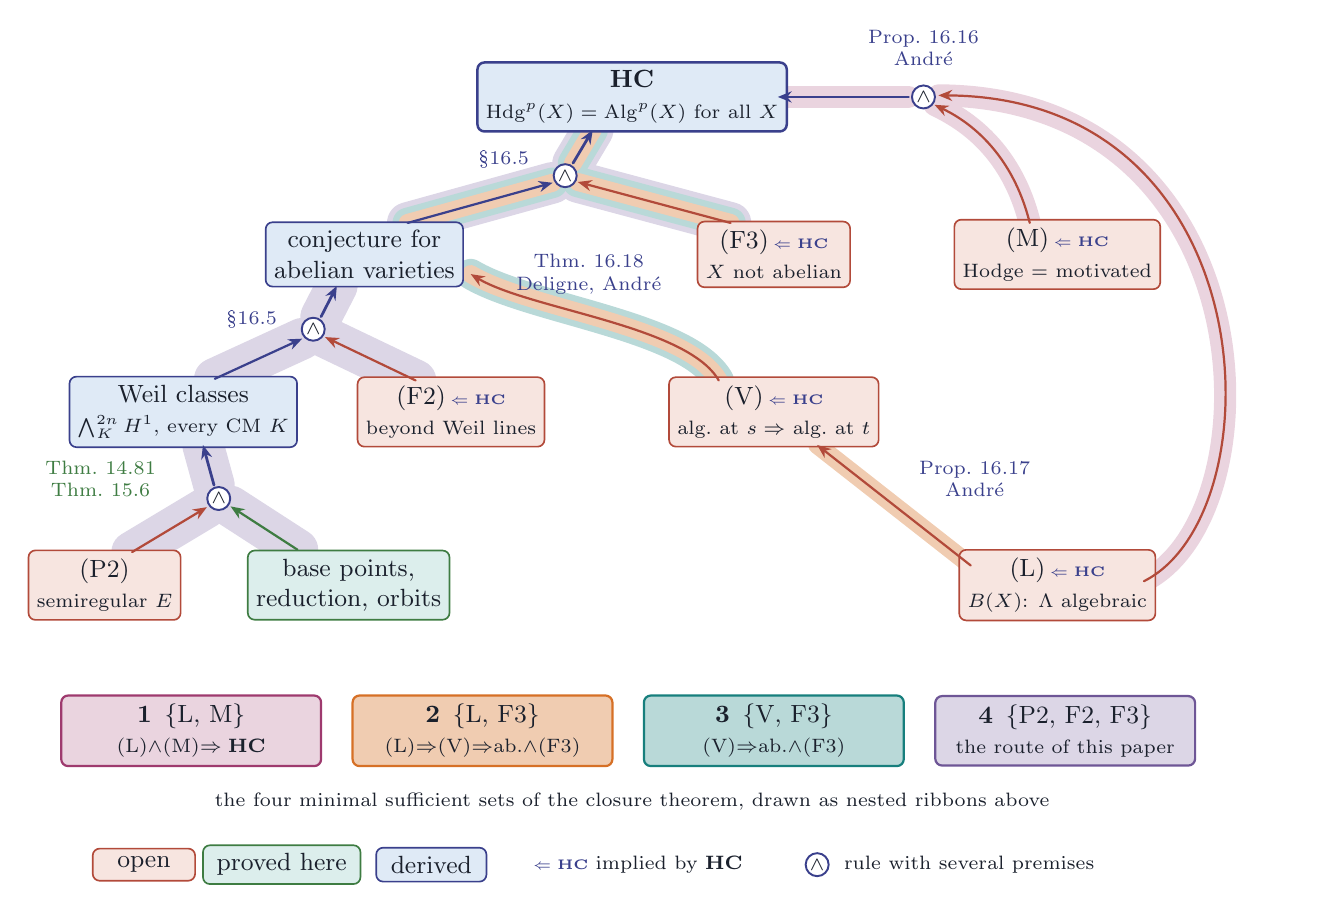
\begin{tikzpicture}[x=1cm,y=1cm,line join=round,line cap=round,
  font=\small,text=PInk]
  \draw[PViolet!24,line width=15.0pt,line cap=round] (-6.35,1.92) -- (-5.40,2.49);
  \draw[PViolet!24,line width=15.0pt,line cap=round] (-4.25,1.95) -- (-5.10,2.50);
  \draw[PViolet!24,line width=15.0pt,line cap=round] (-5.31,2.77) -- (-5.45,3.28);
  \draw[PViolet!24,line width=15.0pt,line cap=round] (-5.30,4.12) -- (-4.19,4.63);
  \draw[PViolet!24,line width=15.0pt,line cap=round] (-2.75,4.10) -- (-3.90,4.65);
  \draw[PViolet!24,line width=15.0pt,line cap=round] (-3.95,4.91) -- (-3.75,5.30);
  \draw[PViolet!24,line width=15.0pt,line cap=round] (-2.85,6.10) -- (-1.01,6.61);
  \draw[PViolet!24,line width=15.0pt,line cap=round] (1.25,6.10) -- (-0.69,6.62);
  \draw[PViolet!24,line width=15.0pt,line cap=round] (-0.75,6.86) -- (-0.50,7.28);
  \draw[PTeal!30,line width=11.0pt,line cap=round] (1.10,4.10) .. controls (0.70,4.80) and (-1.30,5.00) .. (-2.05,5.45);
  \draw[PTeal!30,line width=11.0pt,line cap=round] (-2.85,6.10) -- (-1.01,6.61);
  \draw[PTeal!30,line width=11.0pt,line cap=round] (1.25,6.10) -- (-0.69,6.62);
  \draw[PTeal!30,line width=11.0pt,line cap=round] (-0.75,6.86) -- (-0.50,7.28);
  \draw[PAmber!36,line width=6.5pt,line cap=round] (4.30,1.75) -- (2.35,3.28);
  \draw[PAmber!36,line width=6.5pt,line cap=round] (1.10,4.10) .. controls (0.70,4.80) and (-1.30,5.00) .. (-2.05,5.45);
  \draw[PAmber!36,line width=6.5pt,line cap=round] (-2.85,6.10) -- (-1.01,6.61);
  \draw[PAmber!36,line width=6.5pt,line cap=round] (1.25,6.10) -- (-0.69,6.62);
  \draw[PAmber!36,line width=6.5pt,line cap=round] (-0.75,6.86) -- (-0.50,7.28);
  \draw[PMag!22,line width=8.0pt,line cap=round] (6.50,1.55) .. controls (8.20,2.40) and (8.10,7.70) .. (3.89,7.72);
  \draw[PMag!22,line width=8.0pt,line cap=round] (5.05,6.10) .. controls (4.80,7.10) and (4.15,7.45) .. (3.84,7.60);
  \draw[PMag!22,line width=8.0pt,line cap=round] (3.51,7.70) -- (1.85,7.70);
  \node[draw=PIndigo,fill=WBlue,rounded corners=2.5pt,inner sep=3pt,line width=0.90pt,align=center] at (0.00,7.70) {$\mathbf{HC}$\\{\scriptsize $\Hdg^{p}(X)=\mathrm{Alg}^{p}(X)$ for all $X$}};
  \node[draw=PIndigo,fill=WBlue,rounded corners=2.5pt,inner sep=3pt,line width=0.60pt,align=center] at (-3.40,5.70) {conjecture for\\abelian varieties};
  \node[draw=PClay,fill=WClay,rounded corners=2.5pt,inner sep=3pt,line width=0.60pt,align=center] at (1.80,5.70) {(F3)\hcimp\\{\scriptsize $X$ not abelian}};
  \node[draw=PClay,fill=WClay,rounded corners=2.5pt,inner sep=3pt,line width=0.60pt,align=center] at (5.40,5.70) {(M)\hcimp\\{\scriptsize Hodge $=$ motivated}};
  \node[draw=PIndigo,fill=WBlue,rounded corners=2.5pt,inner sep=3pt,line width=0.60pt,align=center] at (-5.70,3.70) {Weil classes\\{\scriptsize $\textstyle\bigwedge^{2n}_{K}H^{1}$, every CM $K$}};
  \node[draw=PClay,fill=WClay,rounded corners=2.5pt,inner sep=3pt,line width=0.60pt,align=center] at (-2.30,3.70) {(F2)\hcimp\\{\scriptsize beyond Weil lines}};
  \node[draw=PClay,fill=WClay,rounded corners=2.5pt,inner sep=3pt,line width=0.60pt,align=center] at (1.80,3.70) {(V)\hcimp\\{\scriptsize alg.\ at $s\Rightarrow$ alg.\ at $t$}};
  \node[draw=PClay,fill=WClay,rounded corners=2.5pt,inner sep=3pt,line width=0.60pt,align=center] at (5.40,1.50) {(L)\hcimp\\{\scriptsize $B(X)$: $\Lambda$ algebraic}};
  \node[draw=PClay,fill=WClay,rounded corners=2.5pt,inner sep=3pt,line width=0.60pt,align=center] at (-6.70,1.50) {(P2)\\{\scriptsize semiregular $E$}};
  \node[draw=PGrass,fill=WTeal,rounded corners=2.5pt,inner sep=3pt,line width=0.60pt,align=center] at (-3.60,1.50) {base points,\\reduction, orbits};
  \draw[PIndigo,line width=0.80pt,-{Stealth[length=5pt,width=4pt]}] (-2.85,6.10) -- (-1.01,6.61);
  \draw[PClay,line width=0.80pt,-{Stealth[length=5pt,width=4pt]}] (1.25,6.10) -- (-0.69,6.62);
  \draw[PIndigo,line width=1.00pt,-{Stealth[length=5pt,width=4pt]}] (-0.75,6.86) -- (-0.50,7.28);
  \draw[PClay,line width=0.80pt,-{Stealth[length=5pt,width=4pt]}] (5.05,6.10) .. controls (4.80,7.10) and (4.15,7.45) .. (3.84,7.60);
  \draw[PClay,line width=0.80pt,-{Stealth[length=5pt,width=4pt]}] (6.50,1.55) .. controls (8.20,2.40) and (8.10,7.70) .. (3.89,7.72);
  \draw[PIndigo,line width=1.00pt,-{Stealth[length=5pt,width=4pt]}] (3.51,7.70) -- (1.85,7.70);
  \draw[PIndigo,line width=0.80pt,-{Stealth[length=5pt,width=4pt]}] (-5.30,4.12) -- (-4.19,4.63);
  \draw[PClay,line width=0.80pt,-{Stealth[length=5pt,width=4pt]}] (-2.75,4.10) -- (-3.90,4.65);
  \draw[PIndigo,line width=1.00pt,-{Stealth[length=5pt,width=4pt]}] (-3.95,4.91) -- (-3.75,5.30);
  \draw[PClay,line width=0.80pt,-{Stealth[length=5pt,width=4pt]}] (1.10,4.10) .. controls (0.70,4.80) and (-1.30,5.00) .. (-2.05,5.45);
  \draw[PClay,line width=0.80pt,-{Stealth[length=5pt,width=4pt]}] (4.30,1.75) -- (2.35,3.28);
  \draw[PClay,line width=0.80pt,-{Stealth[length=5pt,width=4pt]}] (-6.35,1.92) -- (-5.40,2.49);
  \draw[PGrass,line width=0.80pt,-{Stealth[length=5pt,width=4pt]}] (-4.25,1.95) -- (-5.10,2.50);
  \draw[PIndigo,line width=1.00pt,-{Stealth[length=5pt,width=4pt]}] (-5.31,2.77) -- (-5.45,3.28);
  \node[circle,draw=PIndigo,fill=white,line width=0.7pt,inner sep=0.6pt,font=\scriptsize] at (-0.85,6.70) {$\wedge$};
  \node[circle,draw=PIndigo,fill=white,line width=0.7pt,inner sep=0.6pt,font=\scriptsize] at (3.70,7.70) {$\wedge$};
  \node[circle,draw=PIndigo,fill=white,line width=0.7pt,inner sep=0.6pt,font=\scriptsize] at (-4.05,4.75) {$\wedge$};
  \node[circle,draw=PIndigo,fill=white,line width=0.7pt,inner sep=0.6pt,font=\scriptsize] at (-5.25,2.60) {$\wedge$};
  \node[text=PIndigo,inner sep=1pt,align=center,font=\scriptsize,anchor=east] at (-1.27,6.90) {\S16.5};
  \node[text=PIndigo,inner sep=1pt,align=center,font=\scriptsize,anchor=east] at (-4.47,4.87) {\S16.5};
  \node[text=PIndigo,inner sep=1pt,align=center,font=\scriptsize] at (3.70,8.32) {Prop.~16.16\\Andr\'e};
  \node[text=PIndigo,inner sep=1pt,align=center,font=\scriptsize] at (-0.55,5.45) {Thm.~16.18\\Deligne, Andr\'e};
  \node[text=PIndigo,inner sep=1pt,align=center,font=\scriptsize] at (4.35,2.85) {Prop.~16.17\\Andr\'e};
  \node[text=PGrass,inner sep=1pt,align=center,font=\scriptsize] at (-6.75,2.85) {Thm.~14.81\\Thm.~15.6};
  \node[draw=PMag,fill=PMag!22,rounded corners=2.5pt,inner sep=3pt,line width=0.80pt,align=center,minimum width=3.30cm] at (-5.60,-0.35) {\textbf{1}\enspace$\{$L, M$\}$\\{\scriptsize (L)$\wedge$(M)$\Rightarrow\mathbf{HC}$}};
  \node[draw=PAmber,fill=PAmber!36,rounded corners=2.5pt,inner sep=3pt,line width=0.80pt,align=center,minimum width=3.30cm] at (-1.90,-0.35) {\textbf{2}\enspace$\{$L, F3$\}$\\{\scriptsize (L)$\Rightarrow$(V)$\Rightarrow$ab.$\wedge$(F3)}};
  \node[draw=PTeal,fill=PTeal!30,rounded corners=2.5pt,inner sep=3pt,line width=0.80pt,align=center,minimum width=3.30cm] at (1.80,-0.35) {\textbf{3}\enspace$\{$V, F3$\}$\\{\scriptsize (V)$\Rightarrow$ab.$\wedge$(F3)}};
  \node[draw=PViolet,fill=PViolet!24,rounded corners=2.5pt,inner sep=3pt,line width=0.80pt,align=center,minimum width=3.30cm] at (5.50,-0.35) {\textbf{4}\enspace$\{$P2, F2, F3$\}$\\{\scriptsize the route of this paper}};
  \node[text=PInk,inner sep=1pt,align=center,font=\scriptsize] at (0.00,-1.25) {the four minimal sufficient sets of the closure theorem, drawn as nested ribbons above};
  \node[draw=PClay,fill=WClay,rounded corners=2.5pt,inner sep=3pt,line width=0.60pt,align=center,minimum width=1.30cm] at (-6.20,-2.05) {open};
  \node[draw=PGrass,fill=WTeal,rounded corners=2.5pt,inner sep=3pt,line width=0.60pt,align=center,minimum width=2.00cm] at (-4.45,-2.05) {proved here};
  \node[draw=PIndigo,fill=WBlue,rounded corners=2.5pt,inner sep=3pt,line width=0.60pt,align=center,minimum width=1.40cm] at (-2.55,-2.05) {derived};
  \node[text=PInk,inner sep=1pt,align=center,font=\scriptsize,anchor=west] at (-1.35,-2.05) {\hcimp\ implied by $\mathbf{HC}$};
  \node[circle,draw=PIndigo,fill=white,line width=0.7pt,inner sep=0.6pt,font=\scriptsize] at (2.35,-2.05) {$\wedge$};
  \node[text=PInk,inner sep=1pt,align=center,font=\scriptsize,anchor=west] at (2.65,-2.05) {rule with several premises};
\end{tikzpicture}
\end{document}
